% Бүлэг 1

\chapter{\MakeUppercase{системийн зохиомж}} % Бүлгийн нэр
\label{Chapter3} % Энэ бүлэг рүү ишлэл хийх бол \ref{Chapter1} командыг ашигла 
\pagecolor{white}

%-------------------------------------------------------------------------------

\section{Дэлгэцийн зохиомж}

\begin{figure}[h]
    \centering
    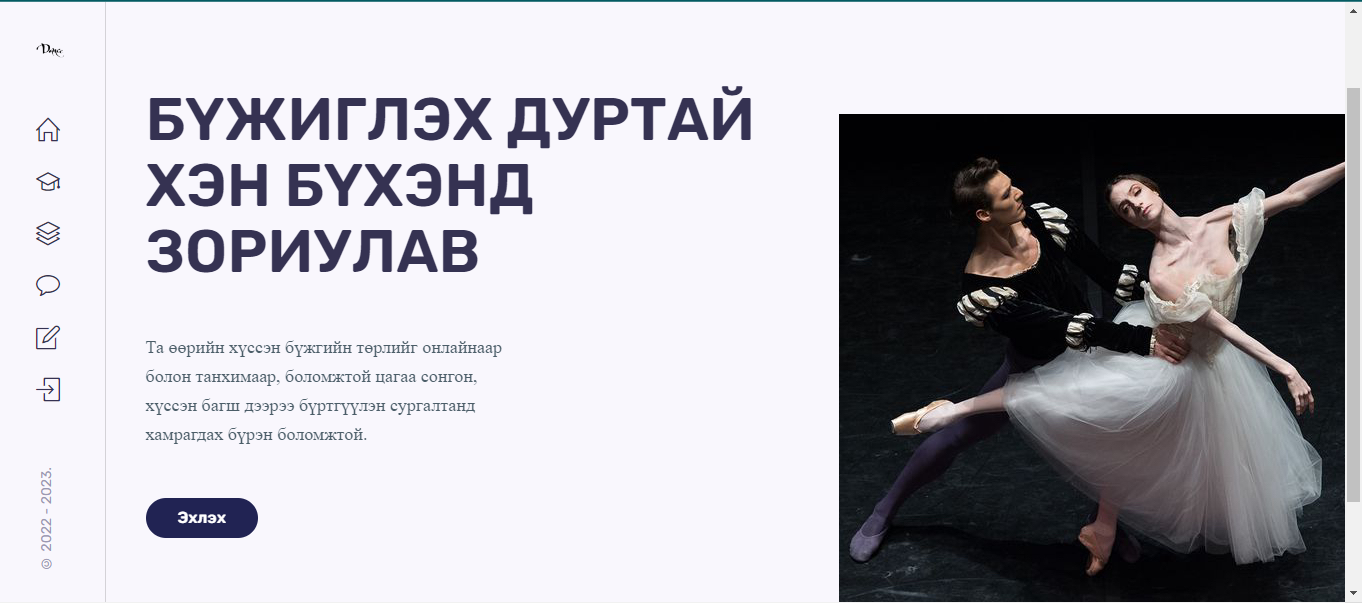
\includegraphics[scale=0.3]{Figures/pic32.png}
    \caption{Вэб сайтын нүүр}
    \label{fig31}
\end{figure}
\begin{figure}[h]
    \centering
    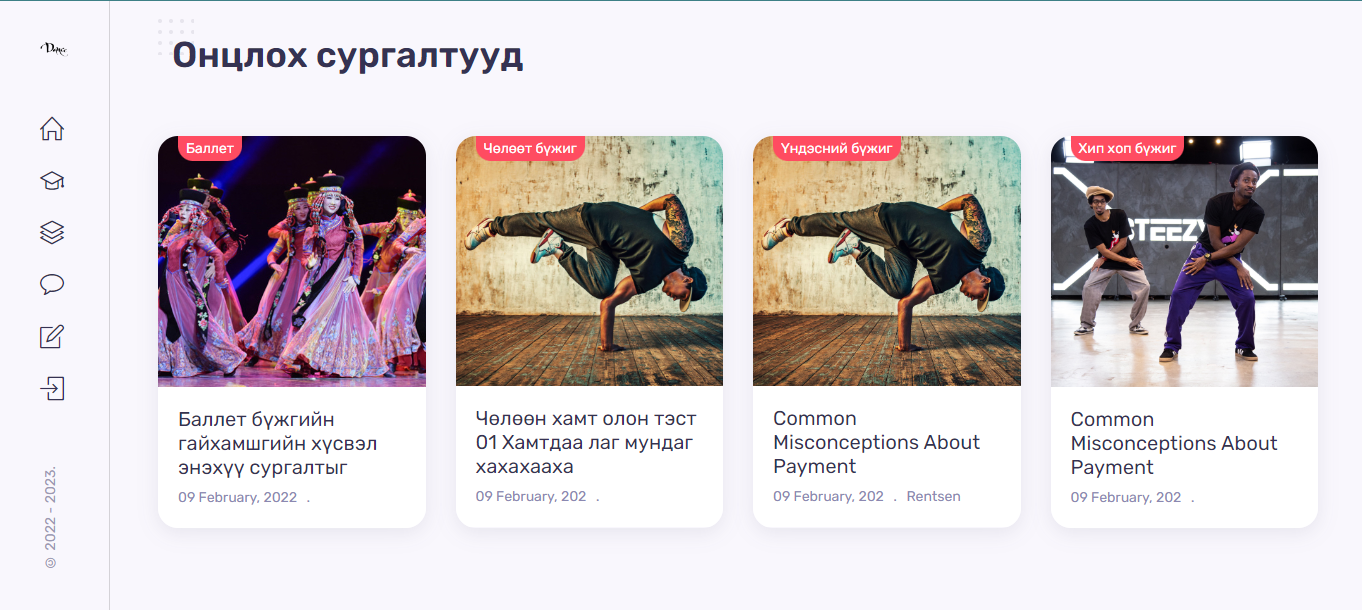
\includegraphics[scale=0.3]{Figures/pic31.png}
    \caption{Онцлох сургалтуудын хуудас}
    \label{fig32}
\end{figure}
\begin{figure}[h]
    \centering
    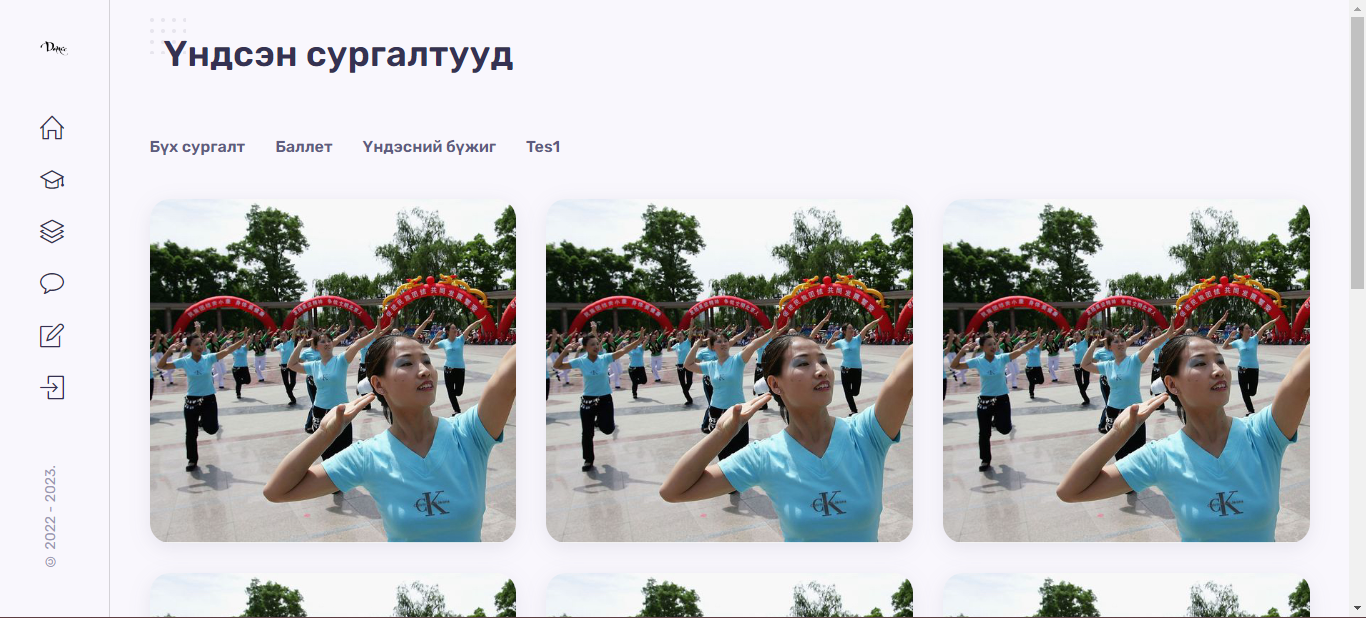
\includegraphics[scale=0.3]{Figures/pic33.png}
    \caption{Сургалтуудын жагсаалтын хуудас}
    \label{fig33}
\end{figure}
\begin{figure}[h]
    \centering
    
\includegraphics[scale=0.3]{Figures/pic35.png}
    \caption{Хэрэглэгчдийн сэтгэгдэл үлдээх хуудас}
    \label{fig34}
\end{figure}
\begin{figure}[h]
    \centering
    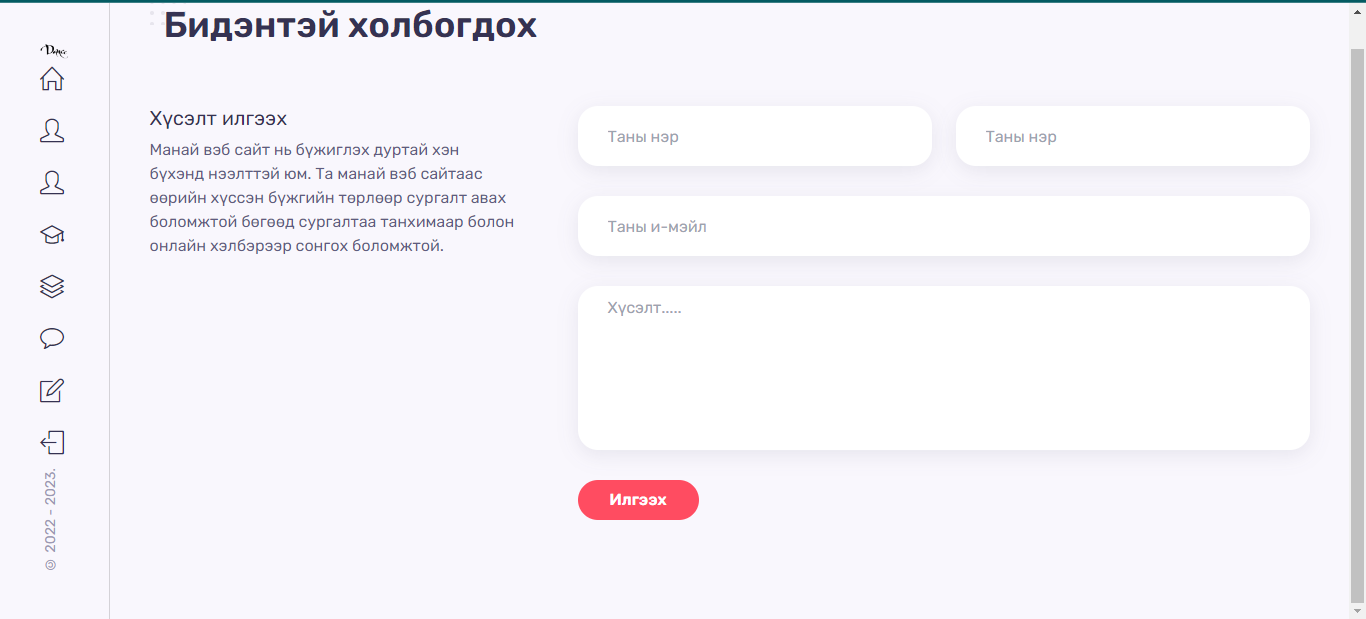
\includegraphics[scale=0.3]{Figures/pic39.png}
    \caption{Бидэнтэй холбогдох хуудас}
    \label{fig35}
\end{figure}
\begin{figure}[h]
    \centering
    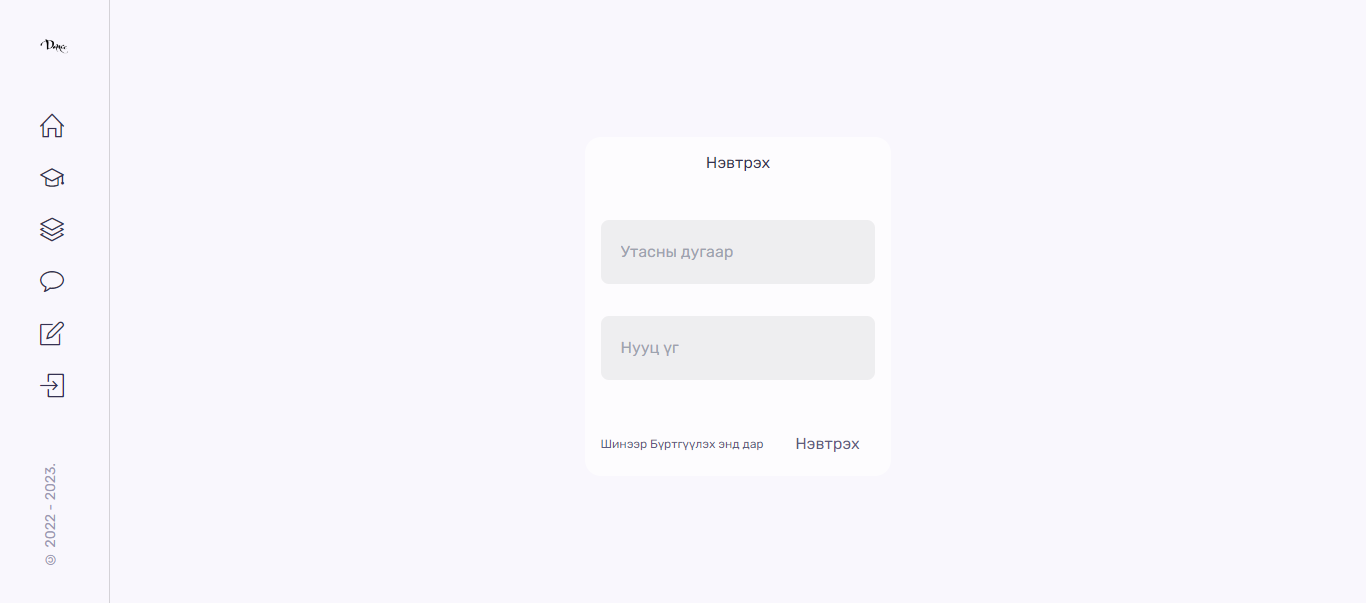
\includegraphics[scale=0.3]{Figures/pic310.png}
    \caption{Нэвтрэх хуудас}
    \label{fig36}
\end{figure}
\begin{figure}[h]
    \centering
    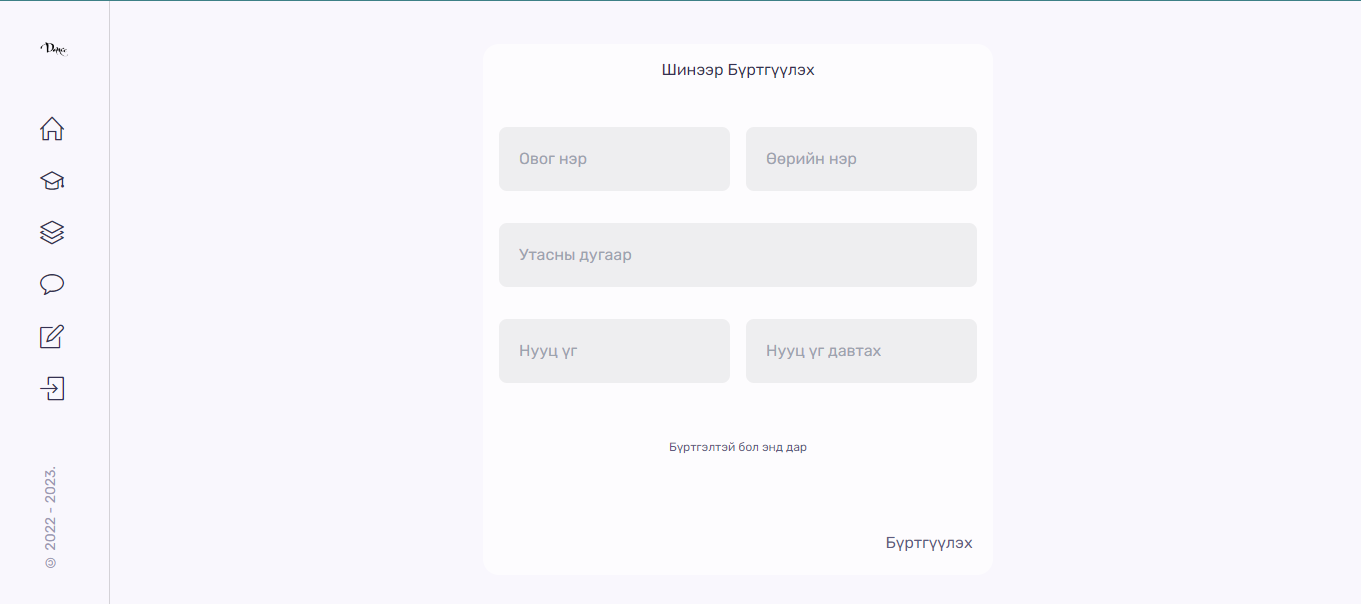
\includegraphics[scale=0.3]{Figures/pic34.png}
    \caption{Шинээр бүртгэл үүсгэх хуудас}
    \label{fig37}
\end{figure}
\begin{figure}[h]
    \centering
    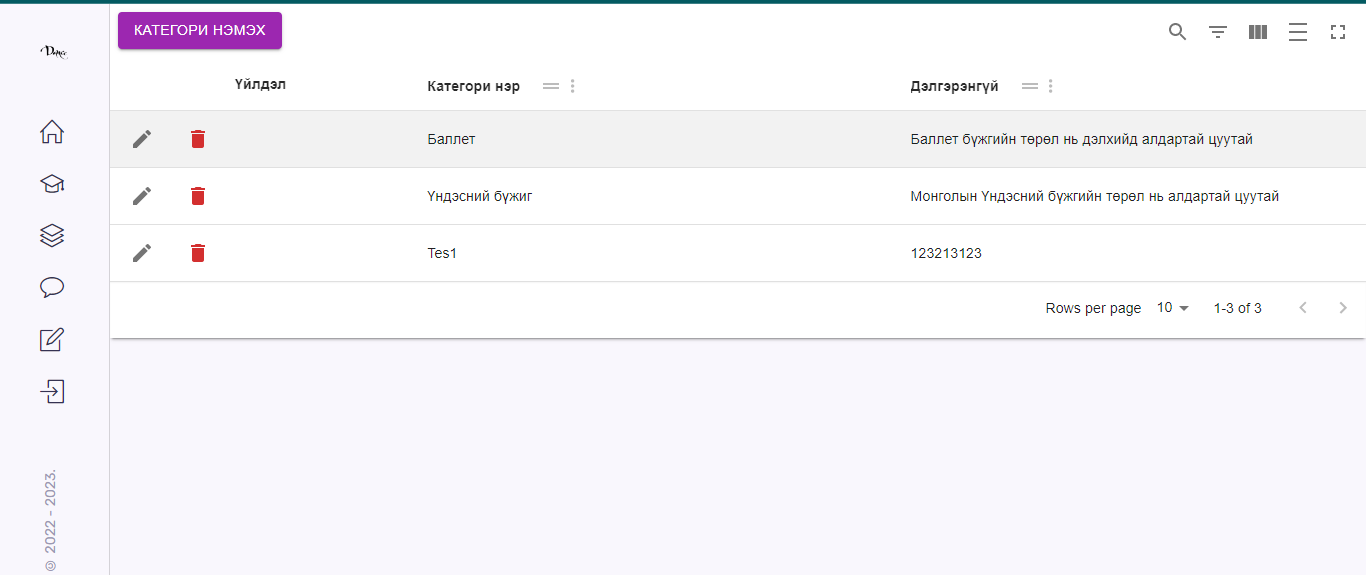
\includegraphics[scale=0.3]{Figures/pic36.png}
    \caption{Админ хуудас}
    \label{fig38}
\end{figure}
\begin{figure}[h]
    \centering
    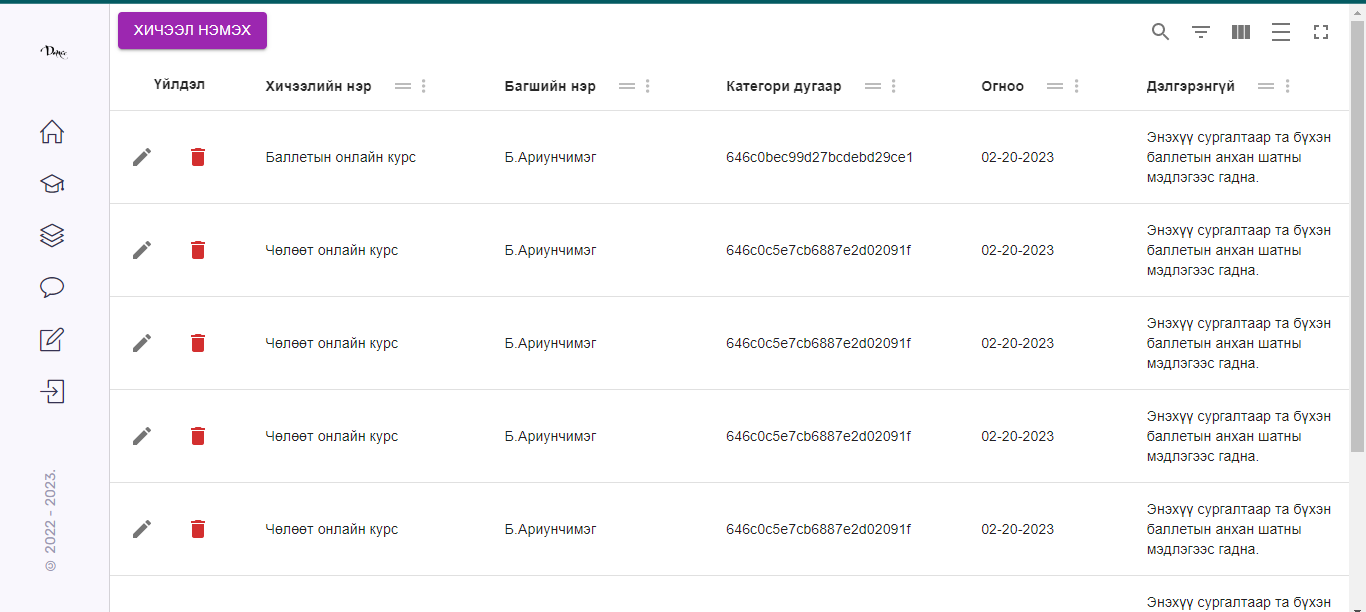
\includegraphics[scale=0.3]{Figures/pic37.png}
    \caption{Админы онлайн хичээл нэмэх хуудас}
    \label{fig39}
\end{figure}
\begin{figure}[h]
    \centering
    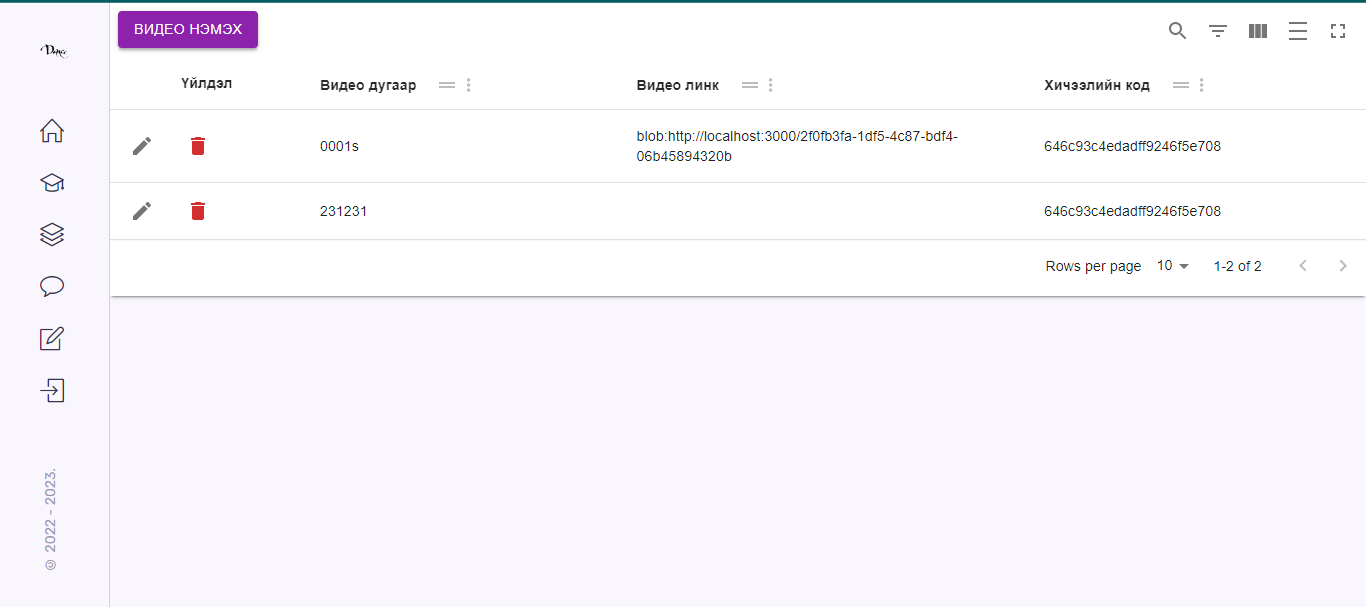
\includegraphics[scale=0.3]{Figures/pic38.png}
    \caption{Админы хичээлд видео нэмэх хуудас}
    \label{fig310}
\end{figure}
\newpage
\section{Үйл ажиллагааны диаграммууд}
\begin{figure}[h]
    \centering
    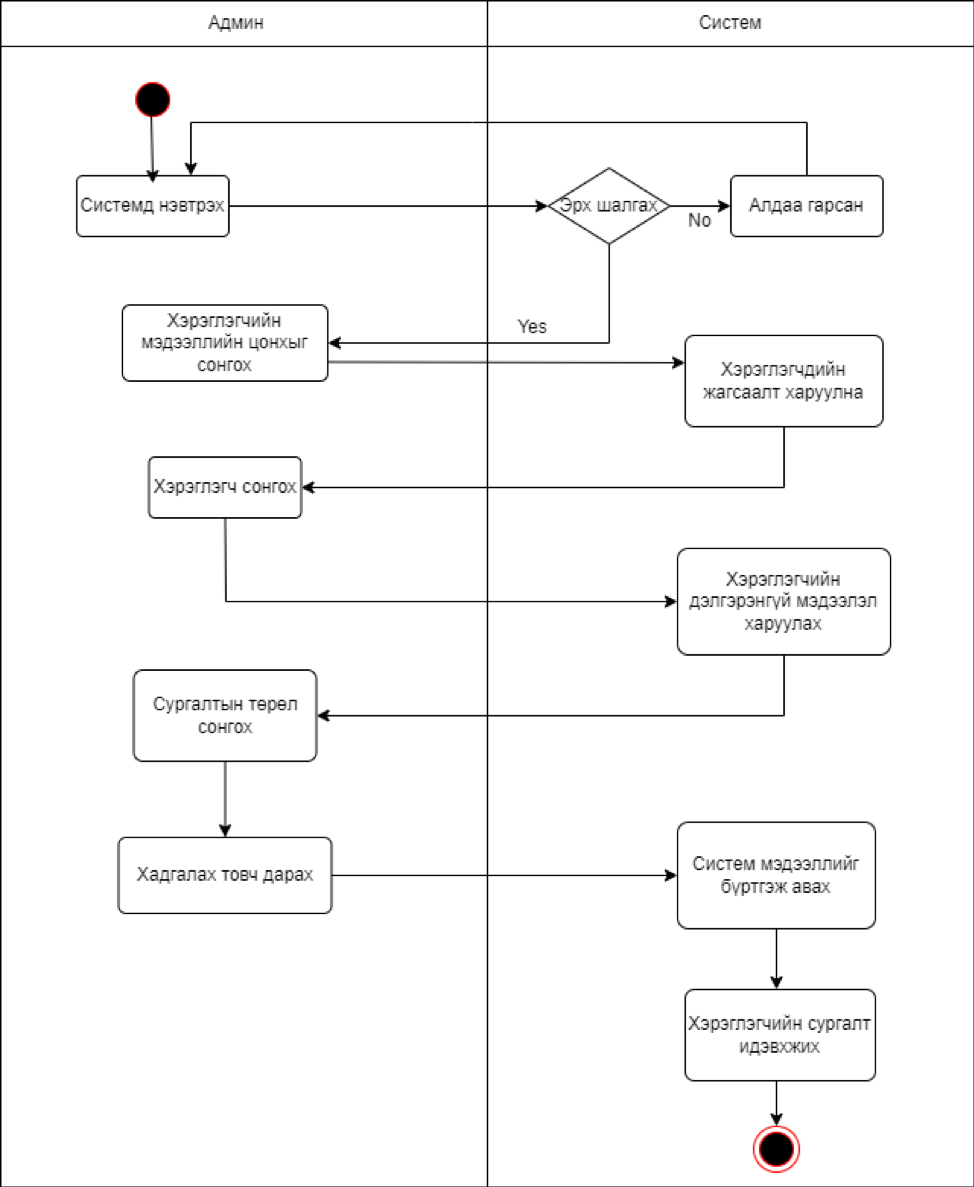
\includegraphics[scale=0.8]{Figures/pic22.png}
    \caption{Үйлчлүүлэгчид эрх олгох үйл ажиллагааны диаграм}
    \label{fig22}
\end{figure}
\begin{figure}[h]
    \centering
    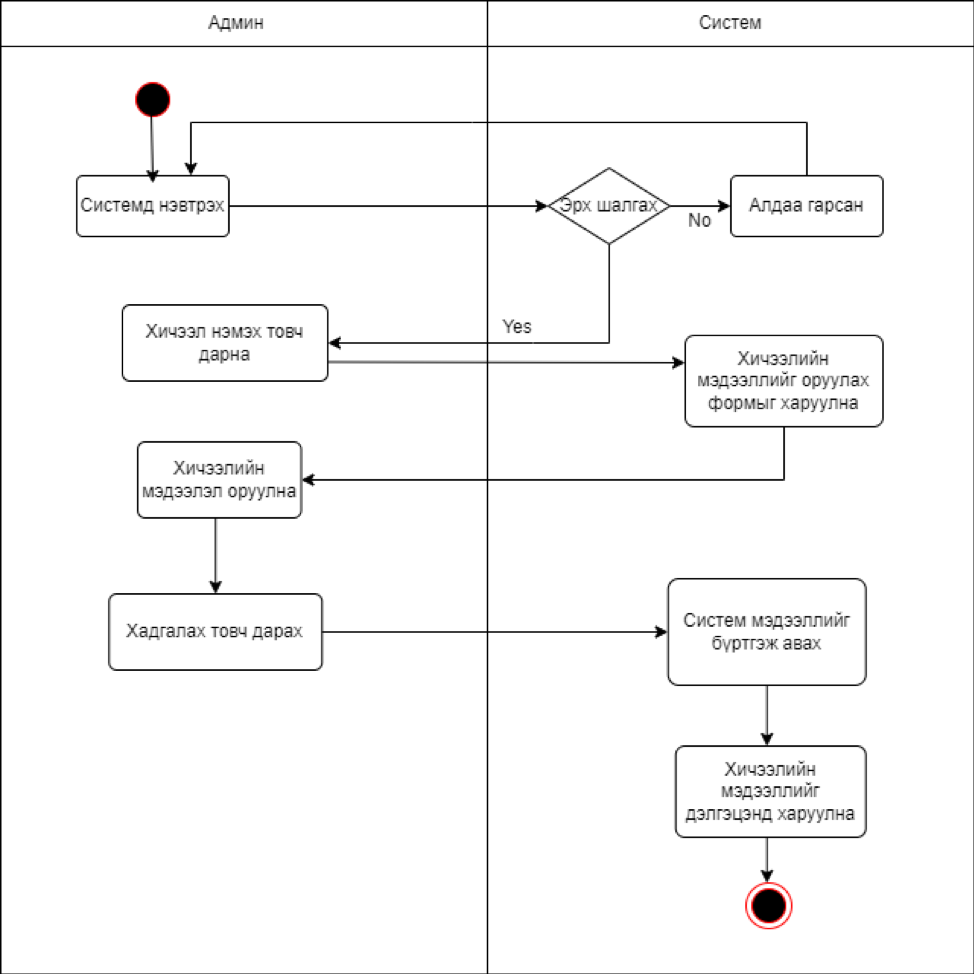
\includegraphics[scale=0.8]{Figures/pic23.png}
    \caption{Хичээл нэмэх үйл ажиллагааны диаграм}
    \label{fig23}
\end{figure}
\begin{figure}[h]
    \centering
    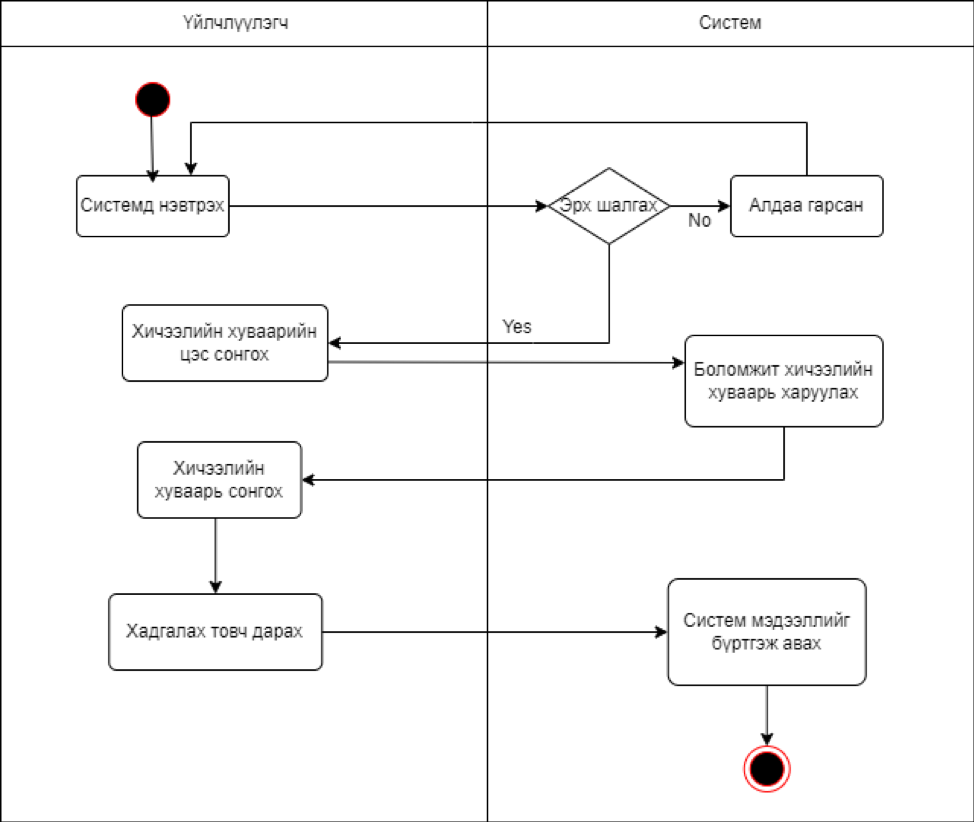
\includegraphics[scale=0.8]{Figures/pic24.png}
    \caption{Хичээлийн хуваарь сонгох үйл ажиллагааны диаграм}
    \label{fig24}
\end{figure}